\begin{proof}[证明]
  $K_p$有$p(p-1)/2$条边,每个哈密顿圈有$p$条边,因此$K_p$最多有$(p-1)/2$个两两无公共边的哈密顿圈。以下只要构造出$(p-1)/2$个两两无公共边的哈密顿圈即可。

  以$p=11$时为例。以下首先画出了第一个哈密顿圈,其顶点序列依次为$1,2,3,4,5,6,7,8,9,10,11,1$。将第一幅图固定不动,顶点的标号依次旋转$\frac{360^\circ}{10}$, $\frac{360^\circ}{10} *2$,$\frac{360^\circ}{10}*3$,$\frac{360^\circ}{10} *4$得到其余的$4$个图,每个图对应一个哈密顿圈。
      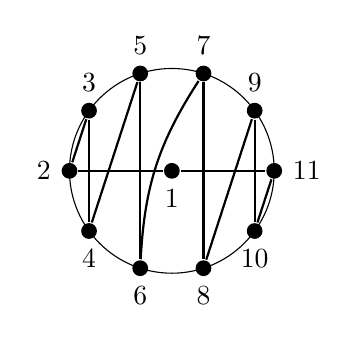
\begin{tikzpicture}[auto,
    specification/.style ={circle, fill, thick, inner sep = 0pt, minimum size=2mm}]
   \node[specification] (A)  [label=-90:$1$] at (0,0)  {};
   \node[specification] (B)  [label=180:$2$] at (180:1.3cm)  {};
   \node[specification] (C)  [label=90:$3$] at (144:1.3cm)  {};
   \node[specification] (E)  [label=90:$5$] at (108:1.3cm)  {};
   \node[specification] (G) [label=90:$7$] at (72:1.3cm)  {};
   \node[specification] (I)  [label=90:$9$] at (36:1.3cm)  {};      
   \node[specification] (K)  [label=0:$11$] at (0:1.3cm)  {};
   \node[specification] (D)  [label=-90:$4$] at (216:1.3cm)  {};
   \node[specification] (F)  [label=-90:$6$] at (252:1.3cm)  {};
   \node[specification] (H) [label=-90:$8$] at (288:1.3cm)  {};
   \node[specification] (J)  [label=-90:$10$] at (324:1.3cm)  {};      
   
   \draw (0,0) circle (1.3cm); 
   \draw[thick] (A) to  (B);
   \draw[thick] (B) to  (C);
   \draw[thick] (C) to  (D);
   \draw[thick] (D) to  (E);
   \draw[thick] (E) to  (F);
   \draw[thick] (F) to [bend left = 15] (G);
   \draw[thick] (G) to  (H);
   \draw[thick] (H) to  (I);
   \draw[thick] (I) to  (J);
   \draw[thick] (J) to  (K);
   \draw[thick] (K) to  (A);
 \end{tikzpicture}
      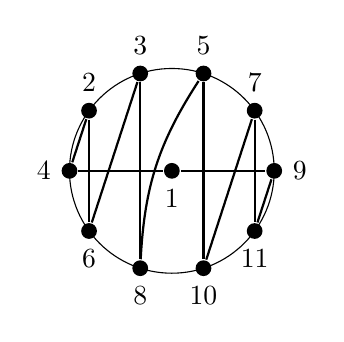
\begin{tikzpicture}[auto,
    specification/.style ={circle, fill, thick, inner sep = 0pt, minimum size=2mm}]
   \node[specification] (A)  [label=-90:$1$] at (0,0)  {};
   \node[specification] (B)  [label=180:$4$] at (180:1.3cm)  {};
   \node[specification] (C)  [label=90:$2$] at (144:1.3cm)  {};
   \node[specification] (E)  [label=90:$3$] at (108:1.3cm)  {};
   \node[specification] (G) [label=90:$5$] at (72:1.3cm)  {};
   \node[specification] (I)  [label=90:$7$] at (36:1.3cm)  {};      
   \node[specification] (K)  [label=0:$9$] at (0:1.3cm)  {};
   \node[specification] (D)  [label=-90:$6$] at (216:1.3cm)  {};
   \node[specification] (F)  [label=-90:$8$] at (252:1.3cm)  {};
   \node[specification] (H) [label=-90:$10$] at (288:1.3cm)  {};
   \node[specification] (J)  [label=-90:$11$] at (324:1.3cm)  {};      
   
   \draw (0,0) circle (1.3cm); 
   \draw[thick] (A) to  (B);
   \draw[thick] (B) to  (C);
   \draw[thick] (C) to  (D);
   \draw[thick] (D) to  (E);
   \draw[thick] (E) to  (F);
   \draw[thick] (F) to [bend left = 15] (G);
   \draw[thick] (G) to  (H);
   \draw[thick] (H) to  (I);
   \draw[thick] (I) to  (J);
   \draw[thick] (J) to  (K);
   \draw[thick] (K) to  (A);
 \end{tikzpicture}
      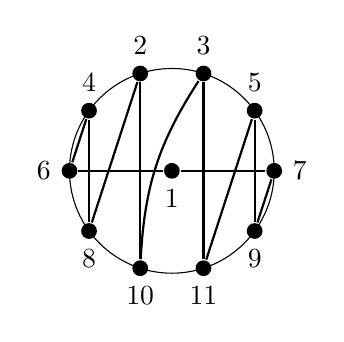
\begin{tikzpicture}[auto,
    specification/.style ={circle, fill, thick, inner sep = 0pt, minimum size=2mm}]
   \node[specification] (A)  [label=-90:$1$] at (0,0)  {};
   \node[specification] (B)  [label=180:$6$] at (180:1.3cm)  {};
   \node[specification] (C)  [label=90:$4$] at (144:1.3cm)  {};
   \node[specification] (E)  [label=90:$2$] at (108:1.3cm)  {};
   \node[specification] (G) [label=90:$3$] at (72:1.3cm)  {};
   \node[specification] (I)  [label=90:$5$] at (36:1.3cm)  {};      
   \node[specification] (K)  [label=0:$7$] at (0:1.3cm)  {};
   \node[specification] (D)  [label=-90:$8$] at (216:1.3cm)  {};
   \node[specification] (F)  [label=-90:$10$] at (252:1.3cm)  {};
   \node[specification] (H) [label=-90:$11$] at (288:1.3cm)  {};
   \node[specification] (J)  [label=-90:$9$] at (324:1.3cm)  {};      
   
   \draw (0,0) circle (1.3cm); 
   \draw[thick] (A) to  (B);
   \draw[thick] (B) to  (C);
   \draw[thick] (C) to  (D);
   \draw[thick] (D) to  (E);
   \draw[thick] (E) to  (F);
   \draw[thick] (F) to [bend left = 15] (G);
   \draw[thick] (G) to  (H);
   \draw[thick] (H) to  (I);
   \draw[thick] (I) to  (J);
   \draw[thick] (J) to  (K);
   \draw[thick] (K) to  (A);
 \end{tikzpicture}
 
      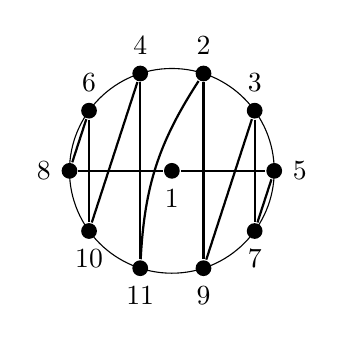
\begin{tikzpicture}[auto,
    specification/.style ={circle, fill, thick, inner sep = 0pt, minimum size=2mm}]
   \node[specification] (A)  [label=-90:$1$] at (0,0)  {};
   \node[specification] (B)  [label=180:$8$] at (180:1.3cm)  {};
   \node[specification] (C)  [label=90:$6$] at (144:1.3cm)  {};
   \node[specification] (E)  [label=90:$4$] at (108:1.3cm)  {};
   \node[specification] (G) [label=90:$2$] at (72:1.3cm)  {};
   \node[specification] (I)  [label=90:$3$] at (36:1.3cm)  {};      
   \node[specification] (K)  [label=0:$5$] at (0:1.3cm)  {};
   \node[specification] (D)  [label=-90:$10$] at (216:1.3cm)  {};
   \node[specification] (F)  [label=-90:$11$] at (252:1.3cm)  {};
   \node[specification] (H) [label=-90:$9$] at (288:1.3cm)  {};
   \node[specification] (J)  [label=-90:$7$] at (324:1.3cm)  {};      
   
   \draw (0,0) circle (1.3cm); 
   \draw[thick] (A) to  (B);
   \draw[thick] (B) to  (C);
   \draw[thick] (C) to  (D);
   \draw[thick] (D) to  (E);
   \draw[thick] (E) to  (F);
   \draw[thick] (F) to [bend left = 15] (G);
   \draw[thick] (G) to  (H);
   \draw[thick] (H) to  (I);
   \draw[thick] (I) to  (J);
   \draw[thick] (J) to  (K);
   \draw[thick] (K) to  (A);
 \end{tikzpicture}
      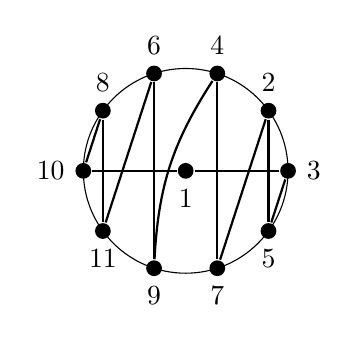
\begin{tikzpicture}[auto,
    specification/.style ={circle, fill, thick, inner sep = 0pt, minimum size=2mm}]
   \node[specification] (A)  [label=-90:$1$] at (0,0)  {};
   \node[specification] (B)  [label=180:$10$] at (180:1.3cm)  {};
   \node[specification] (C)  [label=90:$8$] at (144:1.3cm)  {};
   \node[specification] (E)  [label=90:$6$] at (108:1.3cm)  {};
   \node[specification] (G) [label=90:$4$] at (72:1.3cm)  {};
   \node[specification] (I)  [label=90:$2$] at (36:1.3cm)  {};      
   \node[specification] (K)  [label=0:$3$] at (0:1.3cm)  {};
   \node[specification] (D)  [label=-90:$11$] at (216:1.3cm)  {};
   \node[specification] (F)  [label=-90:$9$] at (252:1.3cm)  {};
   \node[specification] (H) [label=-90:$7$] at (288:1.3cm)  {};
   \node[specification] (J)  [label=-90:$5$] at (324:1.3cm)  {};      
   
   \draw (0,0) circle (1.3cm); 
   \draw[thick] (A) to  (B);
   \draw[thick] (B) to  (C);
   \draw[thick] (C) to  (D);
   \draw[thick] (D) to  (E);
   \draw[thick] (E) to  (F);
   \draw[thick] (F) to [bend left = 15] (G);
   \draw[thick] (G) to  (H);
   \draw[thick] (H) to  (I);
   \draw[thick] (I) to  (J);
   \draw[thick] (J) to  (K);
   \draw[thick] (K) to  (A);
 \end{tikzpicture}

 对于一般的$p$,首先画出第一个哈密顿圈,其顶点序列依次为$1,2,3,\ldots,p,1$,如下图所示。将该图固定不动,顶点的标号依次旋转$\frac{360^\circ}{p-1}$,$\frac{360^\circ}{p-1} *2$,$\ldots$,$\frac{360^\circ}{p-1} *\frac{p-3}{2}$得到其余的$\frac{p-3}{2}$个图,每个图对应一个哈密顿圈。
 
       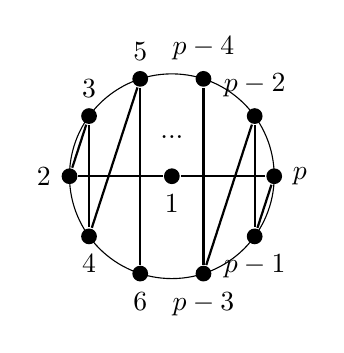
\begin{tikzpicture}[auto,
    specification/.style ={circle, fill, thick, inner sep = 0pt, minimum size=2mm}]
   \node[specification] (A)  [label=-90:$1$] at (0,0)  {};
   \node[specification] (B)  [label=180:$2$] at (180:1.3cm)  {};
   \node[specification] (C)  [label=90:$3$] at (144:1.3cm)  {};
   \node[specification] (E)  [label=90:$5$] at (108:1.3cm)  {};
   \node[specification] (G) [label=90:$p-4$] at (72:1.3cm)  {};
   \node[specification] (I)  [label=90:$p-2$] at (36:1.3cm)  {};      
   \node[specification] (K)  [label=0:$p$] at (0:1.3cm)  {};
   \node[specification] (D)  [label=-90:$4$] at (216:1.3cm)  {};
   \node[specification] (F)  [label=-90:$6$] at (252:1.3cm)  {};
   \node[specification] (H) [label=-90:$p-3$] at (288:1.3cm)  {};
   \node[specification] (J)  [label=-90:$p-1$] at (324:1.3cm)  {};      
   
   \draw (0,0) circle (1.3cm); 
   \draw[thick] (A) to  (B);
   \draw[thick] (B) to  (C);
   \draw[thick] (C) to  (D);
   \draw[thick] (D) to  (E);
   \draw[thick] (E) to  (F);
   % \draw[thick] (F) to [bend left = 15] (G);
   \draw (0cm,0.5cm) node {...};
   \draw[thick] (G) to  (H);
   \draw[thick] (H) to  (I);
   \draw[thick] (I) to  (J);
   \draw[thick] (J) to  (K);
   \draw[thick] (K) to  (A);
 \end{tikzpicture}

\end{proof}